% DSAN architecture figure (adapted from poster_jdd26/figures/dsan_architecture.tex).
% Standalone wrapper stripped; `orange`/`teal` renamed to dsanOrange/dsanTeal to
% avoid clobbering the standard xcolor names used by other figures; the poster's
% custom `back` layer is mapped onto the paper's auto-declared `background` layer.

% ── palette ──
\definecolor{navy}{HTML}{0a2540}
\definecolor{dsanTeal}{HTML}{00d4aa}
\definecolor{tealDk}{HTML}{00b894}
\definecolor{tealBg}{HTML}{e6faf5}
\definecolor{dsanOrange}{HTML}{ff6b35}
\definecolor{orangeDk}{HTML}{e85a25}
\definecolor{orangeBg}{HTML}{fff3ec}
\definecolor{slate}{HTML}{334155}
\definecolor{slateLt}{HTML}{64748b}
\definecolor{border}{HTML}{e2e8f0}
\definecolor{card}{HTML}{ffffff}
\definecolor{bg}{HTML}{f8fafc}
\definecolor{okG}{HTML}{16a34a}
\definecolor{okGBg}{HTML}{dcfce7}
\definecolor{noR}{HTML}{dc2626}
\definecolor{noRBg}{HTML}{fee2e2}

\begin{tikzpicture}[
  >=Stealth,
  % graph mini-nodes
  gn/.style={circle, draw=slateLt, fill=bg, minimum size=3.5pt, inner sep=0pt, line width=0.3pt},
  ga/.style={circle, draw=tealDk, fill=tealBg, minimum size=5pt, inner sep=0pt, line width=0.6pt},
  % flow arrow
  fa/.style={-{Stealth[length=2.8mm, width=2.3mm]}, line width=1.2pt, slateLt},
  fabold/.style={-{Stealth[length=3.2mm, width=2.6mm]}, line width=1.4pt, tealDk!70},
]

% ═══════════════════════════════════════════════
%  LEFT PANEL — Encoder Architecture
% ═══════════════════════════════════════════════

\node[rounded corners=3pt, draw=tealDk, line width=1pt, fill=white, text=tealDk, font=\normalsize\bfseries, inner xsep=8pt, inner ysep=3.5pt] (t1) at (2.6, 0.05) {Architecture};

% Input graphs card
\node[rectangle, rounded corners=3pt,
  minimum width=2.4cm, minimum height=1.45cm,
  draw=border, fill=card,
] (ginbox) at (0.95, -1.25) {};

\node at ([yshift=2.5mm]ginbox.center) {
  \begin{tikzpicture}[scale=0.45]
    \begin{scope}
      \node[ga] (a1) at (0,0) {};
      \node[gn] (a2) at (0.7,0.5) {};
      \node[gn] (a3) at (0.7,-0.5) {};
      \draw[slate!40, line width=0.35pt] (a1)--(a2) (a1)--(a3) (a2)--(a3);
    \end{scope}
    \begin{scope}[shift={(2.0,0)}]
      \node[ga] (b1) at (0,0) {};
      \node[gn] (b2) at (0.6,0.5) {};
      \node[gn] (b3) at (0.6,-0.5) {};
      \node[gn] (b4) at (1.2,0.5) {};
      \node[gn] (b5) at (1.2,-0.5) {};
      \draw[slate!40, line width=0.35pt] (b1)--(b2) (b1)--(b3) (b2)--(b3) (b2)--(b4) (b3)--(b5) (b4)--(b5);
    \end{scope}
  \end{tikzpicture}
};
\node[font=\footnotesize, text=slate, anchor=south] at ([yshift=1mm]ginbox.south) {Input: $G_1,\; G_2$};

% GLASS block
\node[rectangle, rounded corners=3pt,
  minimum width=2.6cm, minimum height=1.45cm,
  draw=orangeDk, line width=1.1pt, fill=white,
  font=\small, text=navy, align=center,
] (glass) at (4.15, -1.25) {\textbf{\color{orangeDk}GLASS}\\[-1pt]Structural Labels\\[0.5pt]
  {\scriptsize\color{slate}anchor + membership}};

% Arrow: input → GLASS
\draw[fa] (ginbox.east) -- (glass.west);

% GNN block
\node[rectangle, rounded corners=4pt,
  minimum width=4.6cm, minimum height=2.7cm,
  draw=tealDk!50, fill=tealBg!40,
  line width=0.8pt,
] (gnnbox) at (2.6, -3.975) {};

% Arrow: GLASS → GNN
\draw[fa] (glass.south) -- (gnnbox.north -| glass.south);

% GNN title
\node[font=\small\bfseries, text=tealDk, anchor=north] at ([yshift=-1.5mm]gnnbox.north) {8$\times$ GraphSAGE GNN};

% Layers inside
\node[rectangle, rounded corners=2pt, minimum width=3.5cm, minimum height=0.48cm,
  draw=border, fill=card, font=\footnotesize, text=slate, align=center,
] (lpre) at ([yshift=3mm]gnnbox.center) {Pre-processing};

\node[rectangle, rounded corners=2pt, minimum width=3.5cm, minimum height=0.48cm,
  draw=tealDk, line width=1pt, fill=white, font=\footnotesize\bfseries, text=tealDk!80!black, align=center,
  below=2.5pt of lpre,
] (lconv) {SAGE Conv $\times 8$ \;{\footnotesize\color{slate}(d=64)}};

\node[rectangle, rounded corners=2pt, minimum width=3.5cm, minimum height=0.48cm,
  draw=dsanOrange!25, fill=orangeBg!60, font=\footnotesize, text=navy, align=center,
  below=2.5pt of lconv,
] (lpost) {Linear + LeakyReLU};

% Skip connection
\draw[slateLt!80, densely dashed, line width=0.5pt, -{Stealth[length=1.4mm]}]
  ([xshift=1.5mm]lpre.east) to[out=0,in=0, looseness=1.4] ([xshift=1.5mm]lpost.east);
\node[font=\scriptsize, text=slateLt, rotate=-90] at ([xshift=5mm]lconv.east) {skip};

% Output
\node[rectangle, rounded corners=3pt,
  minimum width=4.6cm, minimum height=0.65cm,
  draw=navy, line width=1.1pt, fill=white,
  font=\small, text=navy, align=center,
] (out) at (2.6, -6.2) {$\varphi(G_1),\; \varphi(G_2) \in \mathbb{R}^{64}$};

% Arrow: GNN → output
\draw[fabold] (gnnbox.south) -- (out.north);


% ═══════════════════════════════════════════════
%  RIGHT PANEL — Order Embedding Space + Loss
% ═══════════════════════════════════════════════

\node[rounded corners=3pt, draw=navy, line width=1pt, fill=white, text=navy, font=\normalsize\bfseries, inner xsep=8pt, inner ysep=3.5pt] (t2) at (11.1, 0.05) {Order Embedding Space \& Training};

% OES visualization
\node[rectangle, rounded corners=4pt,
  minimum width=4.7cm, minimum height=3.6cm,
  draw=border, fill=card,
] (oesbox) at (8.65, -2.4) {};

\node at ([yshift=-1.5mm]oesbox.center) {
  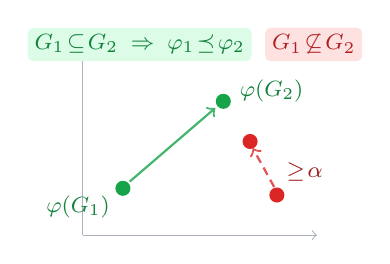
\begin{tikzpicture}[scale=0.85]
    % axes
    \draw[->, slate!40, line width=0.4pt] (-0.3,-0.3) -- (3.2,-0.3);
    \draw[->, slate!40, line width=0.4pt] (-0.3,-0.3) -- (-0.3,2.5);

    % positive pair
    \fill[okG] (0.3,0.4) circle (3.2pt);
    \fill[okG] (1.8,1.7) circle (3.2pt);
    \draw[->, okG!80, line width=0.8pt] (0.4,0.5) -- (1.68,1.6);
    \node[font=\footnotesize, text=okG!80!black, left] at (0.25,0.12) {$\varphi(G_1)$};
    \node[font=\footnotesize, text=okG!80!black, right] at (1.9,1.85) {$\varphi(G_2)$};

    % negative pair
    \fill[noR] (2.6,0.3) circle (3.2pt);
    \fill[noR] (2.2,1.1) circle (3.2pt);
    \draw[->, noR!80, densely dashed, line width=0.8pt] (2.56,0.42) -- (2.24,1.0);
    \node[font=\footnotesize, text=noR!70!black, right] at (2.6,0.65) {$\geq\!\alpha$};

    % legend chips
    \node[font=\footnotesize, text=okG!80!black, fill=okGBg, rounded corners=2pt, inner sep=2.5pt]
      at (0.55, 2.55) {$G_1\!\subseteq\! G_2 \;\Rightarrow\; \varphi_1\!\preceq\!\varphi_2$};
    \node[font=\footnotesize, text=noR!80!black, fill=noRBg, rounded corners=2pt, inner sep=2.5pt]
      at (3.15, 2.55) {$G_1\!\not\subseteq\! G_2$};
  \end{tikzpicture}
};

% Loss function
\node[rectangle, rounded corners=4pt,
  minimum width=4.8cm,
  inner sep=8pt,
  draw=border, fill=bg,
  align=center,
] (lossbox) at (13.7, -2.4) {
  {\small\bfseries\color{navy}Loss Function}\\[5pt]
  $E = \sum_i\big\|\max\big(0,\;\varphi_i^{(1)}\!-\!\varphi_i^{(2)}\big)\big\|^2$\\[7pt]
  $\mathcal{L} = \underbrace{\sum_{\text{\scriptsize pos}} E^+}_{\text{\scriptsize minimize}} \;+\; \underbrace{\sum_{\text{\scriptsize neg}} \log(1\!+\!e^{\,\alpha - E^-})}_{\text{\scriptsize softplus margin}}$
};

% Training info — spans below OES + Loss
\node[font=\footnotesize, text=slate, align=center] (tinfo) at (11.1, -4.75) {
  Trained \textbf{once} on synthetic graphs
};

% ═══════════════════════════════════════════════
%  MATCHING HEAD — the embedding output branches into training (the order
%  embedding space) and inference (the MLP containment classifier).
% ═══════════════════════════════════════════════
\coordinate (br) at (5.65, -6.2);
% stem from the embeddings to the branch point (no arrow head; heads sit at the
% two destinations below)
\draw[line width=1.4pt, tealDk!70, rounded corners=4pt] (out.east) -- (br);
% branch up into the order embedding space (training)
\draw[fabold, rounded corners=4pt] (br) |- (oesbox.west);

% MLP matcher head (binary containment classifier)
\node[rectangle, rounded corners=3pt,
  minimum width=3.0cm, minimum height=1.05cm,
  draw=navy, line width=1.1pt, fill=white,
  font=\small, text=navy, align=center,
] (mlp) at (8.7, -6.2) {\textbf{MLP} matcher head\\[1.5pt]
  {\scriptsize\color{slate}$E \mapsto P(G_1\!\subseteq\! G_2)$}};
% branch right into the matcher head (inference)
\draw[fabold, rounded corners=4pt] (br) -- (mlp.west);

% containment decision
\node[rectangle, rounded corners=3pt,
  minimum width=2.7cm, minimum height=1.05cm,
  draw=okG, line width=1.1pt, fill=okGBg,
  font=\small, text=okG!72!black, align=center,
] (pred) at (12.85, -6.2) {Containment\\[1.5pt]$G_1 \subseteq G_2$};
\draw[-{Stealth[length=3.2mm, width=2.6mm]}, line width=1.4pt, okG!70]
  (mlp.east) -- (pred.west);

% ═══════════════════════════════════════════════
%  Backgrounds
% ═══════════════════════════════════════════════
\begin{pgfonlayer}{background}
  % Left panel bg
  \node[fill=bg, draw=border!50, rounded corners=6pt, line width=0.25pt,
    inner xsep=3mm, inner ysep=2.5mm,
    fit=(t1)(ginbox)(glass)(gnnbox)(out)
  ] {};
  % Right panel bg
  \node[fill=bg, draw=border!50, rounded corners=6pt, line width=0.25pt,
    inner xsep=3mm, inner ysep=2.5mm,
    fit=(t2)(oesbox)(lossbox)(tinfo)
  ] {};
  % Matching band (bottom)
  \node[fill=bg, draw=border!50, rounded corners=6pt, line width=0.25pt,
    inner xsep=3mm, inner ysep=2.5mm,
    fit=(mlp)(pred)
  ] (matchbg) {};
\end{pgfonlayer}

% Reset the bounding box to the actual content (drops stray whitespace that
% would otherwise shift the figure right when scaled to \linewidth).
\pgfresetboundingbox
\useasboundingbox (0.95,0.85) rectangle (17.1,-7.0);

\end{tikzpicture}
